%% LyX 2.0.6 created this file.  For more info, see http://www.lyx.org/.
%% Do not edit unless you really know what you are doing.
\documentclass[english]{article}
\usepackage[T1]{fontenc}
\usepackage[latin9]{inputenc}
\usepackage{url}
\usepackage{graphicx}

\makeatletter

%%%%%%%%%%%%%%%%%%%%%%%%%%%%%% LyX specific LaTeX commands.
%% Because html converters don't know tabularnewline
\providecommand{\tabularnewline}{\\}

\makeatother

\usepackage{babel}
\begin{document}

\title{Soil redox potential as a predictor of benthos species composition
in an intertidal zone}


\author{Rich�l Bilderbeek}
\maketitle
\begin{abstract}
Soil redox potential measurements can be done without much physical
effort in a short amount of time, whereas measuring benthos species
diversity involves more effort and time. This study explored if soil
redox potential can be used as a sole predictor of the abundance of
benthos species. Both variables were measured at an intertidal zone
at Schiermonnikoog at a transect from salt marsh to mudflat. Inundation
was expected to be influential in species composition, and to correct
for this, benthos species and redox values were obtained from two
depths at each site. It was found that redox potential alone cannot
be used as predictor of species composition.
\end{abstract}

\section*{Introduction}
\begin{quote}
He who does not expect will not find out the unexpected, for it is
trackless and unexplored (Heraclitus)
\end{quote}


Species composition is one of the first and most vital pieces of data
a field-based ecological research needs to gather. Any way to reliably
conclude the same information with less work will save researchers
both time and resources. One piece of information that is easy to
obtain is a soil its redox potential. Redox potential is not just
a passive abiotic factor; it is a value is of biological importance
instead. Among others, redox potential can be a measure of oxygen
in the soil, and it is known that plant roots can raise the oxygen
level in the soil (and thus its redox potential) \cite{BlossfeldEtAl2011}.
This positive correlation, however, is not always correct, because
at least one other study finds a negative correlation \cite{DongEtAl2014}.
As far as I know, using redox potential as a predictor of species
being present or not, has not yet been investigated. It might be so,
because no relation is expected. Would this relation be found, those
expectations were incorrect.



This study investigates if soil redox potential can be used as a sole
predictor of benthos species abundance. Or: would it be that some
species abundances are distributed normally around a certain redox
potential?


\section*{Materials and method}



This study was carried out at the intertidal zone of Schiermonnikoog.
In the Southwest of this island, a 2400 meter long transect was set
up, from salt marsh to mudflat. Sample sites were marked with poles,
and occurred every. The elevations of the transect range from 270
cm to -80 cm NAP. All measurements were done at September 9th and
10th. At those days, inundation times of the sample sites ranged from
from 1-80\% of a tidal period.



Soil samples of 20 cm deep were taken at different distances. The
top 5 cm was separated. Both parts of the soil sample were scored
for species. 



Redox values were measured by a potentiometer using 4 platinum-tip
electrodes and a solution of KCl as a reference. The electrodes were
put in at two depths: 2 cm and 10 cm, in this sequence. The potential
read is the value that remained constant, when placing or changing
the electrodes. The values read were transformed to use earth as a
reference point, using the formula $V=1.8847\cdot V_{measured}-53.201$.



Of all collected species, only species with at least 3 individuals
at both depths were taken into account. The minimum value of 3 was
chosen, because it is the minimum number to test for normality. The
requirement for a species to be at two depths is to disrupt the effect
of inundation, as there can be similar redox potentials for different
inundation times. 



For each species, a Shapiro-Wilk normality test was used to determine
if abundance is distributed normally around a certain redox potential.
This test is chosen, as it has the best power for a given significance
\cite{RazaliAndWah2011}.



The script to analyze the data is written in R and can be downloaded
at \url{https://github.com/richelbilderbeek/MemeCourse}.


\section*{Results}

The redox potentials measured can be seen in figure \ref{fig:RedoxPerDistance}.

863 individuals of 18 different species were collected at the site
(see figure \ref{table_species_count_at_depth}). Of these species,
8 species had at least 3 individuals at both depths. Out of these
8 species, only 4 could be used, as not all sites had their redox
potential measured. From the 4 species left, only the 2 species occurring
at multiple redox potentials were analyzed. These two species were
\textit{Hydrobia ulvae} and \textit{Nereis diversicolor}. Figure \ref{fig:SpeciesAbundances}
shows the abundance of both species at different redox potentials.
A Shapiro-Wilk normality test shows that both species have a significant
probability of not following a normal distribution ($p_{Hydrobia}<0.001$,
$p_{Nereis}<0.05$, see table \ref{tab:NormalityTest} for exact values).



\begin{table}
\begin{tabular}{|c|c|c|}
\hline 
Species name & Depth: 2 cm & Depth: 10 cm\tabularnewline
\hline 
\hline 
\textit{Arenicola marina} & 12 & 1\tabularnewline
\hline 
\textit{Bathyporeia} & 2 & 0\tabularnewline
\hline 
\textit{Carcinus maenas} & 3 & 14\tabularnewline
\hline 
\textit{Cerastoderma edule} & 5 & 22\tabularnewline
\hline 
\textit{Crassostrea gigas} & 4 & 6\tabularnewline
\hline 
\textit{Eteone longa} & 0 & 5\tabularnewline
\hline 
\textit{Gammarus locusta} & 1 & 3\tabularnewline
\hline 
\textit{Hemigropsus takanoi} & 4 & 11\tabularnewline
\hline 
\textit{Heteromastus filliformis} & 1 & 13\tabularnewline
\hline 
\textit{Hydrobia ulvae} & 131 & 369\tabularnewline
\hline 
\textit{Lanice conchilega} & 2 & 31\tabularnewline
\hline 
\textit{Littorina littorea} & 11 & 51\tabularnewline
\hline 
\textit{Macoma balthica} & 0 & 31\tabularnewline
\hline 
\textit{Mytilus edulis} & 7 & 78\tabularnewline
\hline 
\textit{Nereis diversicolor} & 14 & 10\tabularnewline
\hline 
\textit{Nereis virens} & 3 & 0\tabularnewline
\hline 
\textit{Scoloplas armiger} & 1 & 16\tabularnewline
\hline 
\textit{Scrobicularia plana} & 1 & 0\tabularnewline
\hline 
\end{tabular}

\caption{\label{table_species_count_at_depth}All 18 species and the number
of individuals found per species per depth. Total number of individuals:
863.}
\end{table}


\begin{figure}
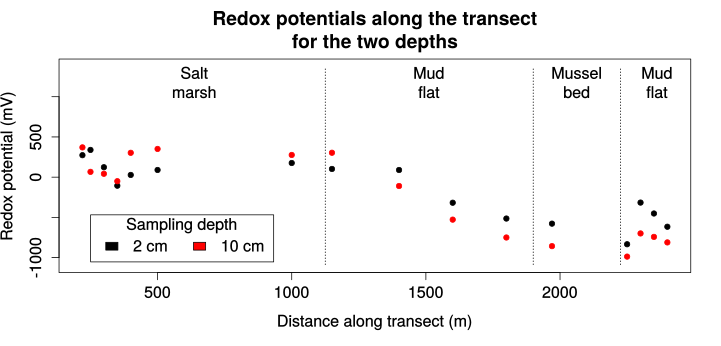
\includegraphics[scale=0.4]{Figure_redox_per_distance}

\caption{\label{fig:RedoxPerDistance}Redox potentials along the transect}
\end{figure}


\begin{figure}
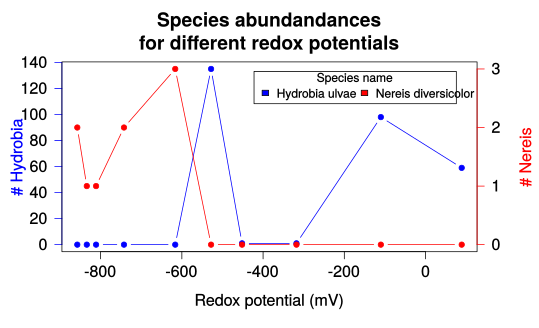
\includegraphics[scale=0.5]{Species_abundances}

\caption{\label{fig:SpeciesAbundances}Number of individuals at the different
redox potentials}
\end{figure}


\begin{table}
\begin{tabular}{|c|c|c|c|}
\hline 
Name & n & p & significance\tabularnewline
\hline 
\hline 
\textit{Hydrobia ulvae} &  & < 2.2e-16 & {*}{*}{*}\tabularnewline
\hline 
\textit{Nereis diversicolor} &  & 0.04965 & {*}\tabularnewline
\hline 
\end{tabular}

\caption{\label{tab:NormalityTest}Shapiro-Wilk normality test of the species
abundances on redox potential. n: number of individuals. p: chance
the species abundances do not follow a normal distribution for a redox
potentia;.}
\end{table}



\section*{Conclusion}

Given a certain redox potential, the abundances of both \textit{Hydrobia
ulvae} and \textit{Nereis diversicolor} can not be predicted, when
assuming their abundance are distributed normally around a certain
redox potential.


\section*{Discussion}

This study makes a strong case that soil redox potential cannot be
used to predict species abundances, for both \textit{Hydrobia ulvae}
and \textit{Nereis diversicolor}. 

As \textit{Hydrobia ulvae} is an epibenthic grazer \cite{Newell1965},
it seems rather obvious that is not influenced by the oxygen level
of the soil underneath it. Less obvious is that individuals were found
in benthos 5 cm below the surface. This finding appears not to be
an experimental error, as \textit{Hydrobia ulvae} is found in deeper
soil samples at multiple distances. 

\textit{Nereis diversicolor} creates burrows in the mud and is a predator
and scavanger \cite{WitteAndWilde1979}. As it does not live in the
soil itself, nor does it feed on something in the soil itself, it
appears rather obvious that also this species is unaffected by soil
redox potential.
\begin{thebibliography}{1}
\bibitem[1]{RazaliAndWah2011}Razali, Nornadiah; Wah, Yap Bee (2011).
Power comparisons of Shapiro\textendash{}Wilk, Kolmogorov\textendash{}Smirnov,
Lilliefors and Anderson\textendash{}Darling tests. Journal of Statistical
Modeling and Analytics 2 (1): 21\textendash{}33

\bibitem[2]{Newell1965}Newell,R.C. (1965). The role of detritus in
the nutrition of two marine deposit-feeders, the prosobranch \textit{Hydrobia
ulvae} and the bivalve \textit{Macoma balthica}. Proc. zool. Soc.
Lond. 144, 25-45 

\bibitem[3]{Rauschenplat1901}Rauschenplat, E (1901). Ueber die Nahrung
von Thierer aus der Kielerbucht. Wiss. Meeresunters. 5(2):85-151. 

\bibitem[4]{BlossfeldEtAl2011}Blossfeld, S; Gansert, D; Thiele B;
Kuhn AJ; L�sch R (2011). The dynamics of oxygen concentration, pH
value, and organic acids in the rhizosphere of Juncus spp. Soil Biology
\& Biochemistry 43:1186-1197

\bibitem[5]{DongEtAl2014}Dong, B; Han, R; Wang, G; Cao, X (2014).
O2, pH, and Redox Potential Microprofiles around \textit{Potamogeton
malaianus} Measured Using Microsensors. PLoS ONE 9(7): e101825. doi:10.1371/journal.pone.0101825

\bibitem[6]{WitteAndWilde1979}Witte, F; Wilde, de, PAWJ (1979). On
the ecological relation between \textit{Nereis diversicolor} and juvenile
\textit{Arenicola marina}. Netherlands Journal of Sea Research 13(3/4):
394-405

\end{thebibliography}

\subsection*{Appendix}

?Documentation of R code?
\end{document}
